\chapter{Структура FILE}


\begin{lstlisting}[caption={\text{Структура FILE}}]
typedef struct _IO_FILE FILE;
struct _IO_FILE
{
	int _flags;		/* High-order word is _IO_MAGIC; rest is flags. */
	
	/* The following pointers correspond to the C++ streambuf protocol. */
	char *_IO_read_ptr;	/* Current read pointer */
	char *_IO_read_end;	/* End of get area. */
	char *_IO_read_base;	/* Start of putback+get area. */
	char *_IO_write_base;	/* Start of put area. */
	char *_IO_write_ptr;	/* Current put pointer. */
	char *_IO_write_end;	/* End of put area. */
	char *_IO_buf_base;	/* Start of reserve area. */
	char *_IO_buf_end;	/* End of reserve area. */
	
	/* The following fields are used to support backing up and undo. */
	char *_IO_save_base; /* Pointer to start of non-current get area. */
	char *_IO_backup_base;  /* Pointer to first valid character of backup area */
	char *_IO_save_end; /* Pointer to end of non-current get area. */
	
	struct _IO_marker *_markers;
	
	struct _IO_FILE *_chain;
	
	int _fileno;
	int _flags2;
	__off_t _old_offset; /* This used to be _offset but it's too small.  */
	
	/* 1+column number of pbase(); 0 is unknown. */
	unsigned short _cur_column;
	signed char _vtable_offset;
	char _shortbuf[1];
	
	_IO_lock_t *_lock;
	#ifdef _IO_USE_OLD_IO_FILE
};
\end{lstlisting}

\chapter{Программа №1}

\begin{lstlisting}[caption={\text{Программа №1}}]
#include <fcntl.h>
#include <stdio.h>

int main() {
	// have kernel open connection to file alphabet.txt
	int fd = open("alphabet.txt", O_RDONLY);
	
	// create two a C I/O buffered streams using the above connection
	FILE *fs1 = fdopen(fd, "r");
	char buff1[20];
	setvbuf(fs1, buff1, _IOFBF, 20);
	
	FILE *fs2 = fdopen(fd, "r");
	char buff2[20];
	setvbuf(fs2, buff2, _IOFBF, 20);
	
	// read a char & write it alternatingly from fs1 and fs2
	int flag1 = 1, flag2 = 2;
	while (flag1 == 1 || flag2 == 1) {
		char c;
		
		flag1 = fscanf(fs1, "%c", &c);
		if (flag1 == 1) fprintf(stdout, "%c", c);
		
		flag2 = fscanf(fs2, "%c", &c);
		if (flag2 == 1) fprintf(stdout, "%c", c);
	}
	
	return 0;
}
\end{lstlisting}

Результат работы: aubvcwdxeyfzghijklmnopqrst

\begin{lstlisting}[caption={\text{Программа №1 (многопоточная)}}]
#include <fcntl.h>
#include <pthread.h>
#include <stdio.h>
#define BUF_SIZE 20
#define FILENAME "alphabet.txt"

void *t1_run(void *args) {
	int *fd = (int *)args;
	FILE *fs1 = fdopen(*fd, "r");
	char buff1[BUF_SIZE];
	setvbuf(fs1, buff1, _IOFBF, BUF_SIZE);
	int flag = 1;
	char c;
	while ((flag = fscanf(fs1, "%c", &c)) == 1)
	fprintf(stdout, "%c", c);
	return NULL;
}

void *t2_run(void *args) {
	int *fd = (int *)args;
	FILE *fs2 = fdopen(*fd, "r");
	char buff2[BUF_SIZE];
	setvbuf(fs2, buff2, _IOFBF, BUF_SIZE);
	int flag = 1;
	char c;
	while ((flag = fscanf(fs2, "%c", &c)) == 1)
	fprintf(stdout, "%c", c);
	return NULL;
}

int main() {
	pthread_t t1, t2;
	int fd = open(FILENAME, O_RDONLY);
	
	pthread_create(&t1, NULL, t1_run, &fd);
	pthread_create(&t2, NULL, t2_run, &fd);
	
	pthread_join(t1, NULL);
	pthread_join(t2, NULL);
	return 0;
}
\end{lstlisting}

Результаты работы (несколько запусков программы): 
\begin{itemize}
\item abcdefghijklmnopqrstuvwxyz
\item abuvwxyzcdefghijklmnopqrst
\item aubvcwdxeyfzghijklmnopqrst
\end{itemize}


В программе файл открывается \textit{один} раз системным вызовом \texttt{open}. Системный вызов \texttt{open} возвращает дескриптор файла типа \texttt{int}. Возвращенный номер \texttt{fd} -- индекс дескриптора открытого файла в таблице дискрипторов файлов процесса.
	
 Функция \texttt{fdopen()} создаёт указатель на структуру \texttt{FILE}. Поле \texttt{\_fileno} в \texttt{struct \_IO\_FILE} содержит номер дескриптора, который вернула функция \texttt{open()}.
	
 Функция \texttt{setvbuf()} явно задает размер буффера в 20 байт и меняет тип буферизации	(для \texttt{fs1} и \texttt{fs2}) на полный.
	
 При первом вызове функции \texttt{fscanf()} в цикле (для \texttt{fs1}) \texttt{buff1} будет заполнен полностью -- первыми 20 символами (буквами алфавита). \texttt{f\_pos} в структуре \texttt{struct\_file} открытого файла увеличится на 20.
	
 При втором вызове \texttt{fscanf()} в цикле (для \texttt{fs2}) буффер \texttt{buff2} будет заполнен оставшимися 6 символами (начиная с \texttt{f\_pos}).



\begin{table}[H]
	\centering
	\begin{tabular}{p{1\linewidth}}
		\centering
		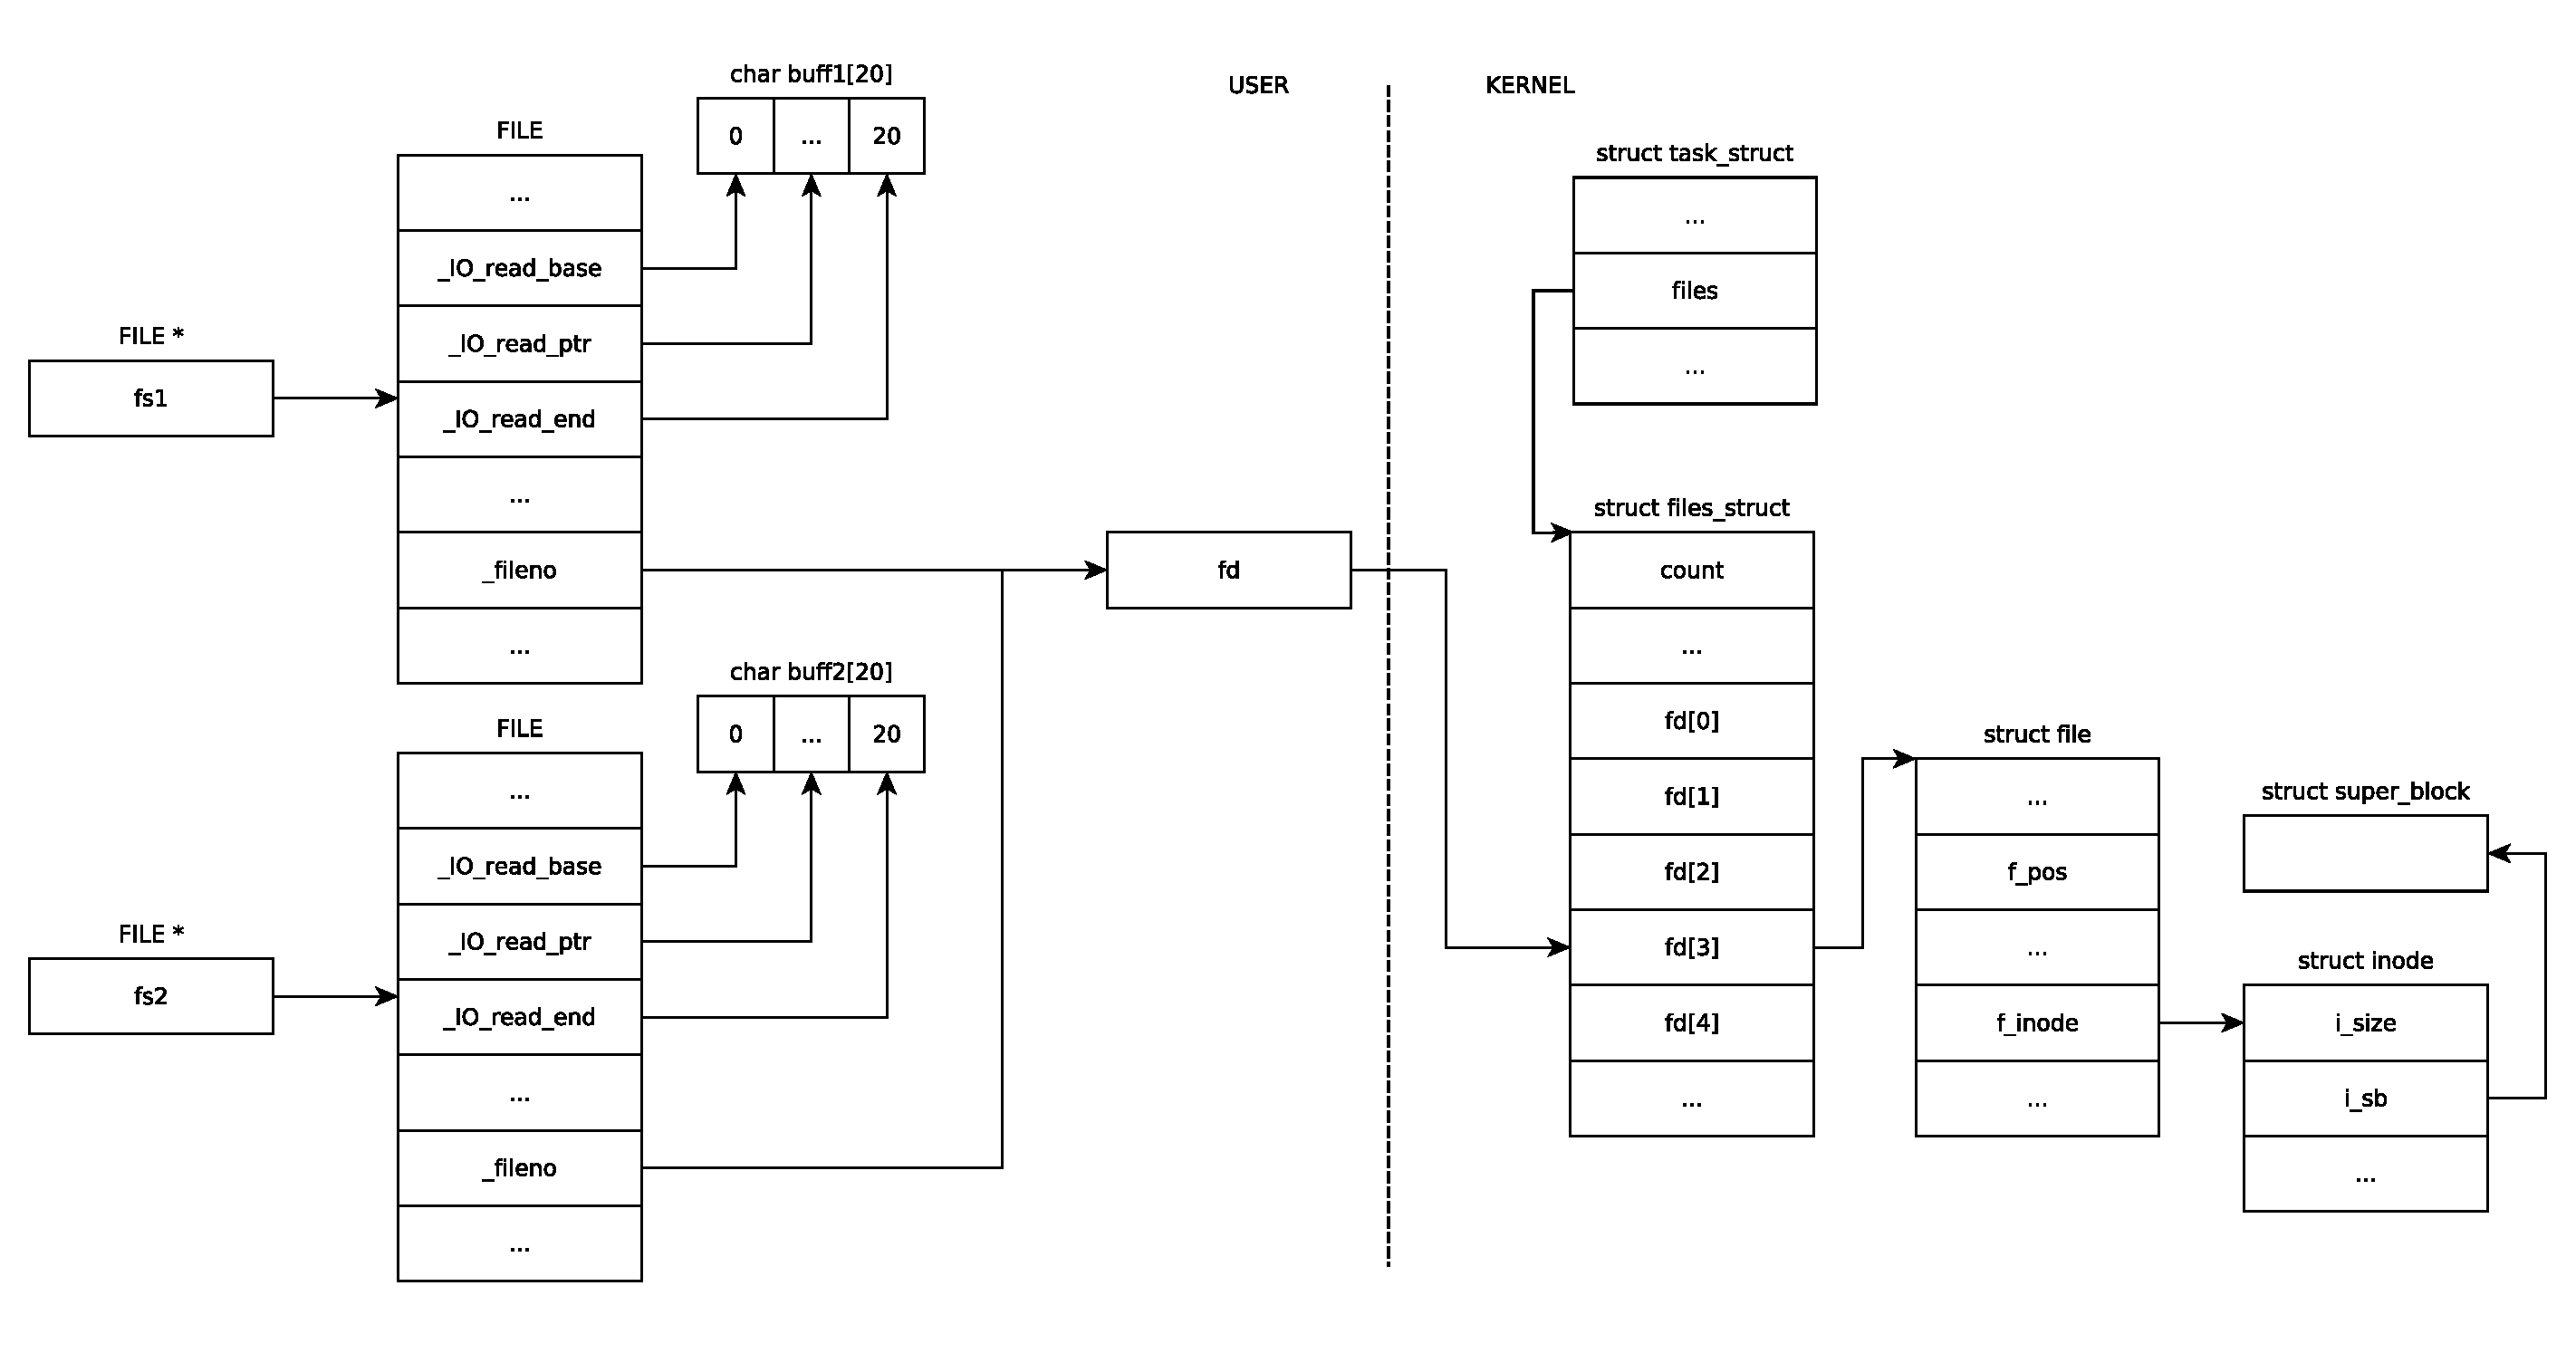
\includegraphics[width=1.0\linewidth]{assets/scheme1.pdf}
		\captionof{figure}{Используемые структуры}
		\label{img:1}
	\end{tabular}
\end{table}

\section{Программа №2}


\begin{lstlisting}[caption={\text{Программа №2}}]
#include <fcntl.h>
#include <unistd.h>
int main() {
	int fd1 = open("alphabet.txt", O_RDONLY);
	int fd2 = open("alphabet.txt", O_RDONLY);
	char c;
	while (read(fd1, &c, 1) == 1 && read(fd2, &c, 1) == 1) {
		write(1, &c, 1);
		write(1, &c, 1);
	}
	return 0;
}
\end{lstlisting}

Результат работы: aabbccddeeffgghhiijjkkllmmnnooppqqrrssttuuvvwwxxyyzz

\begin{lstlisting}[caption={\text{Программа №2 (многопоточная)}}]
	#include <fcntl.h>
	#include <pthread.h>
	#include <stdio.h>
	#define BUF_SIZE 20
	#define FILENAME "alphabet.txt"
	
	void *t1_run(void *args) {
		int *fd = (int *)args;
		FILE *fs1 = fdopen(*fd, "r");
		char buff1[BUF_SIZE];
		setvbuf(fs1, buff1, _IOFBF, BUF_SIZE);
		int flag = 1;
		char c;
		while ((flag = fscanf(fs1, "%c", &c)) == 1)
		fprintf(stdout, "%c", c);
		return NULL;
	}
	
	void *t2_run(void *args) {
		int *fd = (int *)args;
		FILE *fs2 = fdopen(*fd, "r");
		char buff2[BUF_SIZE];
		setvbuf(fs2, buff2, _IOFBF, BUF_SIZE);
		int flag = 1;
		char c;
		while ((flag = fscanf(fs2, "%c", &c)) == 1)
		fprintf(stdout, "%c", c);
		return NULL;
	}
	
	int main() {
		pthread_t t1, t2;
		int fd = open(FILENAME, O_RDONLY);
		
		pthread_create(&t1, NULL, t1_run, &fd);
		pthread_create(&t2, NULL, t2_run, &fd);
		
		pthread_join(t1, NULL);
		pthread_join(t2, NULL);
		return 0;
	}
\end{lstlisting}

Результаты работы (несколько запусков программы): 
\begin{itemize}
	\item aabcdbefcgdheifjgkhlimjnkolpmqnrosptqurvswtxuyvzwxyz
	\item aabbcdcedfefgghhiijjkkllmmnnooppqqrrssttuuvvwwxxyyzz
	\item aabbccddeeffgghihjijkkllmmnnopoqprqsrtsutvuwvxwyxzyz
\end{itemize}


 Функция \texttt{open()} создает файловый дескриптор, два раза для одного и того же файла, поэтому в программе существует две различные \texttt{struct file}, но ссылающиеся на один	и тот же \texttt{struct inode}.
	
	 Из-за того что структуры разные (у каждой структуры свое поле \texttt{f\_pos}), посимвольная печать дважды выведет содержимое файла в формате <<\texttt{aabbcc...}>> (в случае однопоточной реализации).
	
	В случае многопоточной реализации, потоки выполняются с разной скоростью и символы перемешаются.



\begin{table}[H]
	\centering
	\begin{tabular}{p{1\linewidth}}
		\centering
		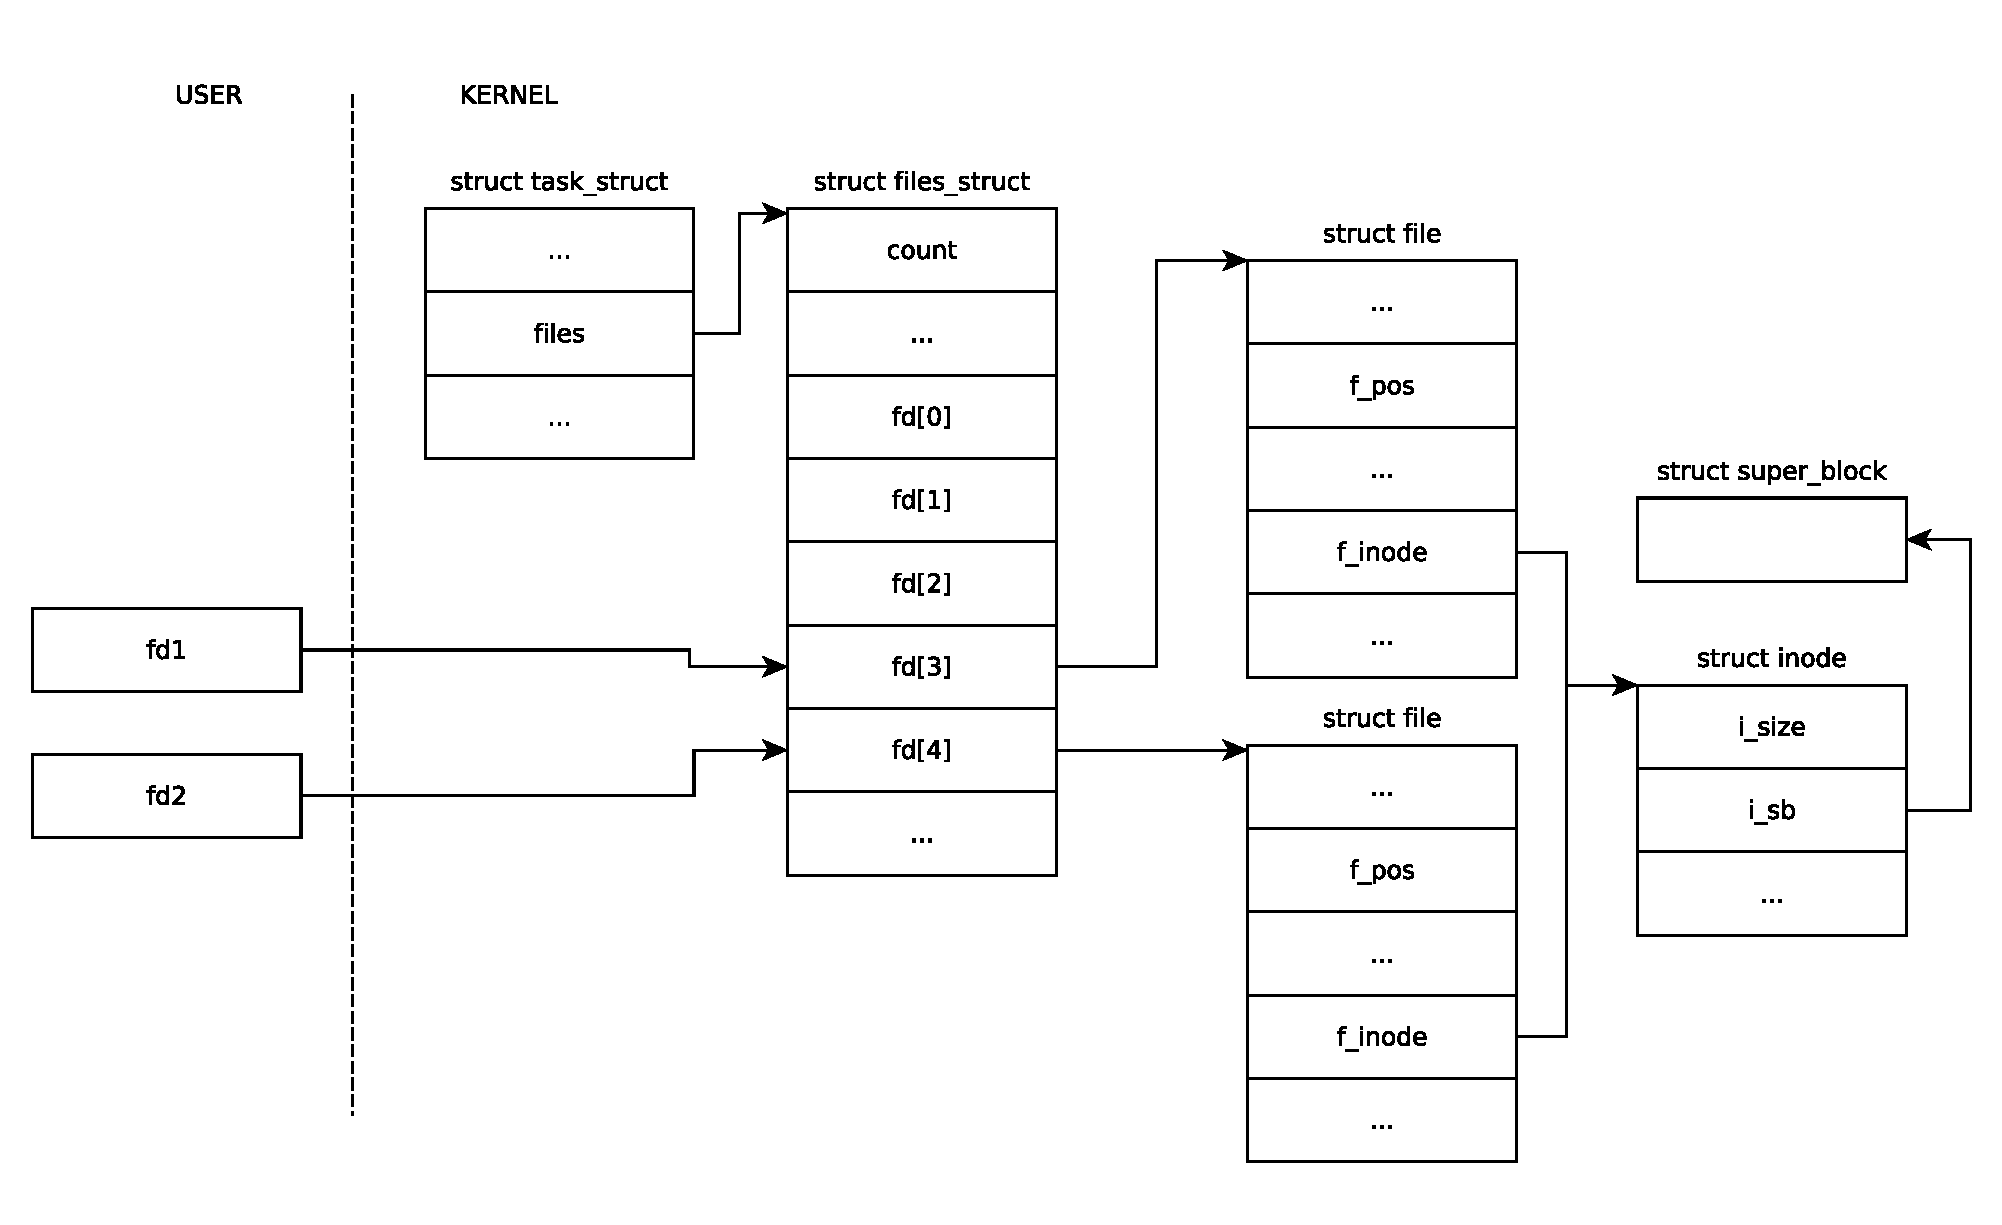
\includegraphics[width=1.0\linewidth]{assets/scheme2.pdf}
		\captionof{figure}{Используемые структуры}
		\label{img:2}
	\end{tabular}
\end{table}

\section{Программа №3}


\begin{lstlisting}[caption={\text{Программа №3}}]
#include <fcntl.h>
#include <stdio.h>
#include <unistd.h>

#define FILENAME "out.txt"

int main() {
	FILE *f1 = fopen(FILENAME, "w");
	FILE *f2 = fopen(FILENAME, "w");
	
	for (char c = 'a'; c <= 'z'; c++) {
		if (c % 2) {
			fprintf(f1, "%c", c);
		} else {
			fprintf(f2, "%c", c);
		}
	}
	
	fclose(f1);
	fclose(f2);
	
	return 0;
}
\end{lstlisting}

Результат работы: bdfhjlnprtvxz

\begin{lstlisting}[caption={\text{Программа №3 (многопоточная)}}]
#include <fcntl.h>
#include <pthread.h>
#include <stdio.h>
#include <unistd.h>

#define FILENAME "out.txt"

void *t1_run(void *args) {
	FILE *f = fopen(FILENAME, "w");
	
	for (char c = 'a'; c <= 'z'; c += 2) {
		fprintf(f, "%c", c);
	}
	
	fclose(f);
	
	return NULL;
}

void *t2_run(void *args) {
	FILE *f = fopen(FILENAME, "w");
	
	for (char c = 'b'; c <= 'z'; c += 2) {
		fprintf(f, "%c", c);
	}
	
	fclose(f);
	
	return NULL;
}

int main() {
	pthread_t t1, t2;
	pthread_create(&t1, NULL, t1_run, NULL);
	pthread_create(&t2, NULL, t2_run, NULL);
	
	pthread_join(t1, NULL);
	pthread_join(t2, NULL);
	
	return 0;
}
\end{lstlisting}

Результаты работы (несколько запусков программы): 
\begin{itemize}
	\item acegikmoqsuwy
	\item bdfhjlnprtvxz
\end{itemize}

 Файл открывается на запись два раза функцией \texttt{fopen()}.
 
  Из-за того \texttt{f\_pos} независимы для каждого дескриптора файла, запись в файл будет производится с нулевой позиции.

Функция \texttt{fprintf()} предоставляет буферизованный вывод.

 Изначально информация пишется в буфер, а из буфера в файл если произошло одно из
событий:
\begin{enumerate}
	\item буффер полон
	\item вызвана функция \texttt{fclose()}
	\item вызвана функция \texttt{fflush()}
\end{enumerate}

В случае нашей программы, информация в файл запишется в результате вызова функции \texttt{fclose()}. Запись в файл происходит в результате вызова функции fclose. При вызове fclose() для fs1 буфер для fs1 записывается в файл. При вызове fclose() для fs2, все содержимое файла очищается, а в файл записывается содержимое буфера для fs2. В итоге произошла утеря данных, в файле окажется только содержимое буфера для fs2. Чтобы этого избеать, необходимо использовать open() с флагом O\_APPEND. Если этот флаг установлен, то каждой операции добавления гарантируется неделимость. 
 



\begin{table}[H]
	\centering
	\begin{tabular}{p{1\linewidth}}
		\centering
		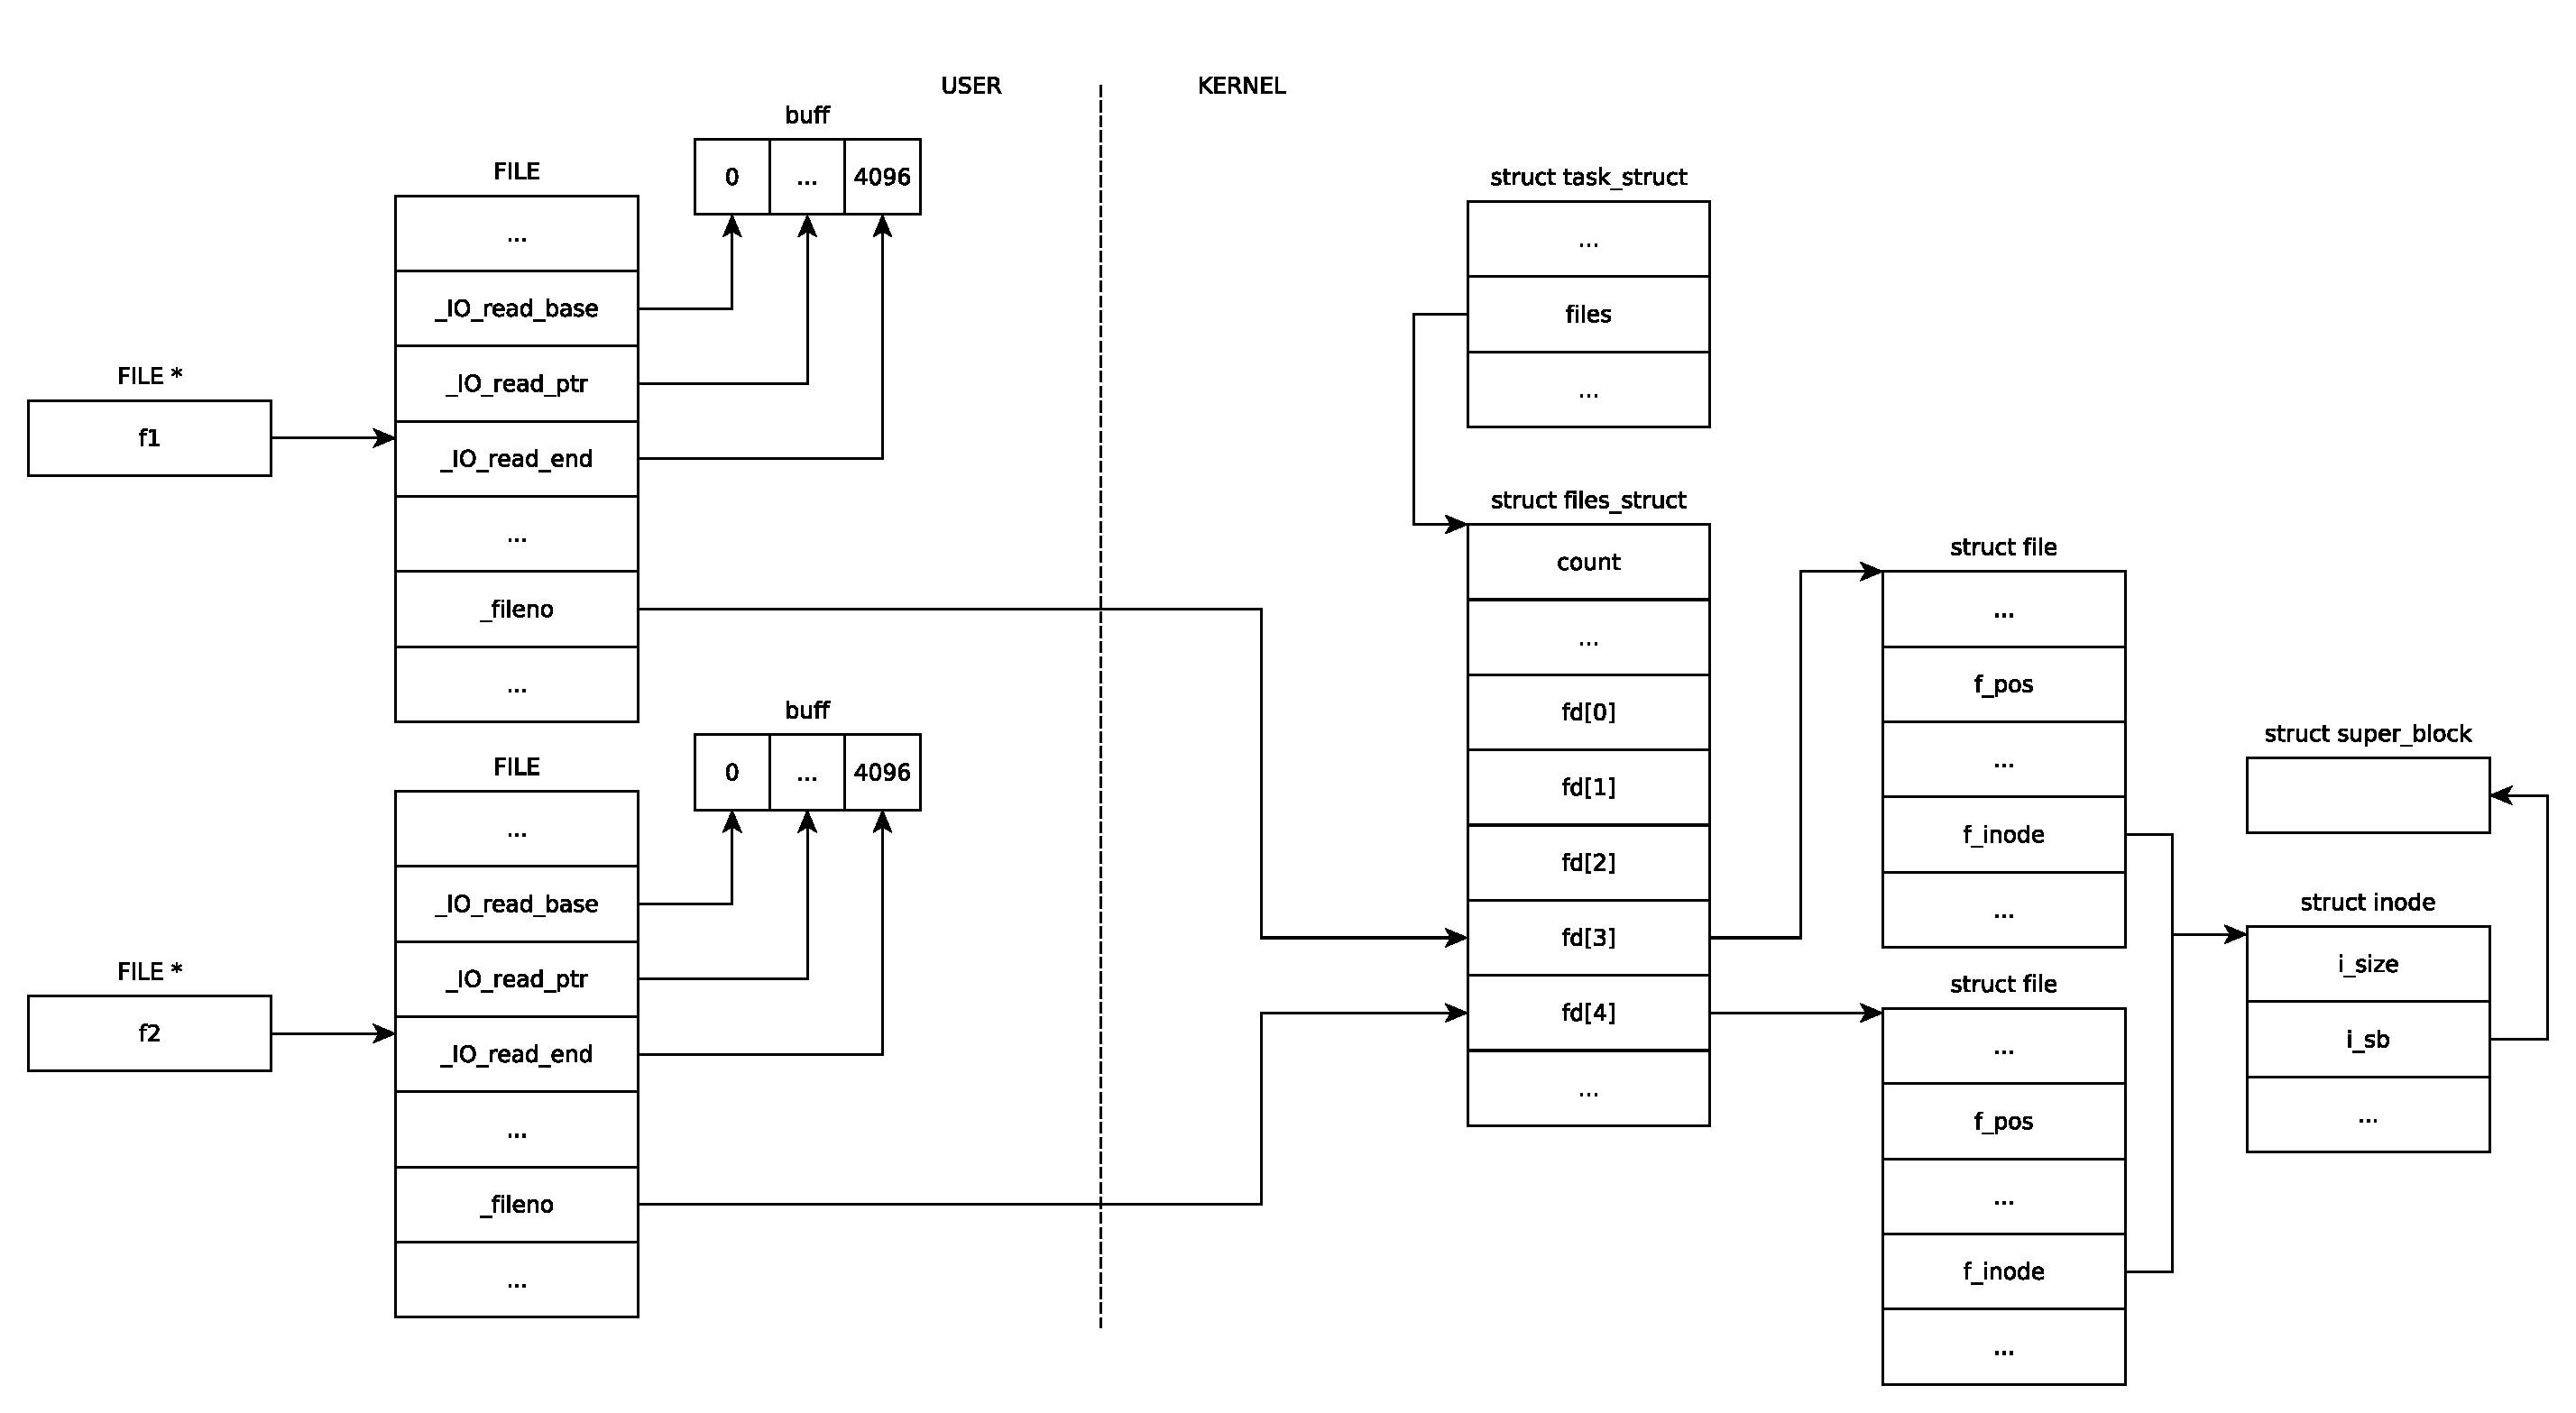
\includegraphics[width=1.0\linewidth]{assets/scheme3.pdf}
		\captionof{figure}{Используемые структуры}
		\label{img:3}
	\end{tabular}
\end{table}

\section{Программа №3 (с open, read, write)}
\begin{lstlisting}[caption={\text{Программа №3 (с open, read, write)}}]
#include <fcntl.h>
#include <stdio.h>
#include <unistd.h>

#define FILENAME "out.txt"

int main() {
	int f1 = open(FILENAME, O_WRONLY | O_CREAT);
	int f2 = open(FILENAME, O_WRONLY | O_CREAT);
	
	for (char c = 'a'; c <= 'z'; c++) {
		if (c % 2) {
			write(f1, &c, 1);
		} else {
			write(f2, &c, 1);
		}
	}
	
	close(f1);
	close(f2);
	return 0;
}
\end{lstlisting}

Результат работы: bdfhjlnprtvxz

\begin{lstlisting}[caption={\text{Программа №3 (с open, read, write) (многопоточная)}}]
#include <fcntl.h>
#include <pthread.h>
#include <stdio.h>
#include <unistd.h>

#define FILENAME "out.txt"

void *t1_run(void *args) {
	int f = open(FILENAME, O_WRONLY | O_CREAT);
	
	for (char c = 'a'; c <= 'z'; c += 2) {
		write(f, &c, 1);
	}
	
	close(f);
	
	return NULL;
}

void *t2_run(void *args) {
	int f = open(FILENAME, O_WRONLY | O_CREAT);
	
	for (char c = 'b'; c <= 'z'; c += 2) {
		write(f, &c, 1);
	}
	
	close(f);
	
	return NULL;
}

int main() {
	pthread_t t1, t2;
	pthread_create(&t1, NULL, t1_run, NULL);
	pthread_create(&t2, NULL, t2_run, NULL);
	pthread_join(t1, NULL);
	pthread_join(t2, NULL);
	return 0;
}
\end{lstlisting}

Результаты работы (несколько запусков программы): 
\begin{itemize}
	\item acegikmoqsuwy
	\item bdfhjlnprtvxz
\end{itemize}











